\documentclass[../../LearnCpp.tex]{subfiles}

\begin{document}

\asubsection{8}{Virtual base classes}

17.9 章节中提到了继承中的“菱形问题”,这章节将恢复这个问题的讨论。

\begin{lstlisting}[language=C++]
#include <iostream>

class PoweredDevice
{
public:
    PoweredDevice(int power)
    {
    std::cout << "PoweredDevice: " << power << '\n';
    }
};

class Scanner: public PoweredDevice
{
public:
    Scanner(int scanner, int power)
        : PoweredDevice{ power }
    {
    std::cout << "Scanner: " << scanner << '\n';
    }
};

class Printer: public PoweredDevice
{
public:
    Printer(int printer, int power)
        : PoweredDevice{ power }
    {
    std::cout << "Printer: " << printer << '\n';
    }
};

class Copier: public Scanner, public Printer
{
public:
    Copier(int scanner, int printer, int power)
        : Scanner{ scanner, power }, Printer{ printer, power }
    {
    }
};
\end{lstlisting}

尽管预期继承的图像是这样:

\begin{figure}[ht]
    \centering
    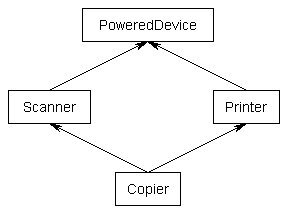
\includegraphics[width=10cm]{\subfix{../images/PoweredDevice}}
    \label{fig:PoweredDevice recap}
    \caption{PoweredDevice recap}
\end{figure}

如果创建了一个 \acode{Copier} 类的对象,默认会得到两份 \acode{PoweredDevice} 类 --
一个给 \acode{Printer},另一个给 \acode{Scanner}。

\begin{figure}[ht]
    \centering
    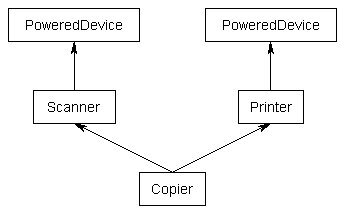
\includegraphics[width=10cm]{\subfix{../images/PoweredDevice2}}
    \label{fig:PoweredDevice2}
    \caption{PoweredDevice2}
\end{figure}

\begin{lstlisting}[language=C++]
int main()
{
    Copier copier{ 1, 2, 3 };

    return 0;
}
\end{lstlisting}

打印:

\begin{lstlisting}[language=C++]
PoweredDevice: 3
Scanner: 1
PoweredDevice: 3
Printer: 2
\end{lstlisting}

可以看到,\acode{PoweredDevice} 被构造了两次。

虽然以上是经常需要的,但是其它时候可以只有一个副本的 \acode{PoweredDevice} 被 \acode{Printer} 与 \acode{Scanner} 共享。

\subsubsection*{虚基类}

为了共享一个基类,只需要简单的在派生类的继承列表前加上“virtual”关键字即可。
这样创建的被称为\textbf{虚基类} virtual base class,意味着仅会有一个基对象。
基对象被所有基础树种的对象共享,并且只会被构造一次。

\begin{lstlisting}[language=C++]
class PoweredDevice
{
};

class Scanner: virtual public PoweredDevice
{
};

class Printer: virtual public PoweredDevice
{
};

class Copier: public Scanner, public Printer
{
};
\end{lstlisting}

现在可以创建一个 \acode{Copier} 类对象,
并且只会拥有一个被 \acode{Printer} 与 \acode{Scanner} 共享的 \acode{PoweredDevice} 副本。

然而这会带来另一个问题:
如果 \acode{Scanner} 和 \acode{Printer} 共享一个 \acode{PoweredDevice} 基类,
那么谁去负责构建它?
答案是 \acode{Copier},其构造函数负责创建 \acode{PoweredDevice}。
因此,这是 \acode{Copier} 被允许直接调用非直接父类的构造函数的时刻:

\begin{lstlisting}[language=C++]
#include <iostream>

class PoweredDevice
{
public:
    PoweredDevice(int power)
    {
        std::cout << "PoweredDevice: " << power << '\n';
    }
};

class Scanner: virtual public PoweredDevice // 注意:PoweredDevice 现在是虚基类
{
public:
    Scanner(int scanner, int power)
        : PoweredDevice{ power } // 该行需要用于 Scanner 对象的创建,但是本例忽略
    {
        std::cout << "Scanner: " << scanner << '\n';
    }
};

class Printer: virtual public PoweredDevice // 注意:PoweredDevice 现在是虚基类
{
public:
    Printer(int printer, int power)
        : PoweredDevice{ power } // 该行需要用于 Printer 对象的创建,但是本例忽略
    {
        std::cout << "Printer: " << printer << '\n';
    }
};

class Copier: public Scanner, public Printer
{
public:
    Copier(int scanner, int printer, int power)
        : PoweredDevice{ power }, // PoweredDevice 在这里构造
        Scanner{ scanner, power }, Printer{ printer, power }
    {
    }
};

int main()
{
    Copier copier{ 1, 2, 3 };

    return 0;
}
\end{lstlisting}

打印:

\begin{lstlisting}
PoweredDevice: 3
Scanner: 1
Printer: 2
\end{lstlisting}

可以看到 \acode{PoweredDevice} 仅被构建了一次。

有几个细节需要注意。

首先,虚基类总是创建在非虚基类之前,这样可以确保所有基类在派生类创建之前被创建。

其次,注意 \acode{Printer} 与 \acode{Scanner} 构造函数仍需要调用 \acode{PoweredDevice} 构造函数。
当创建 \acode{Copier} 的实例时,这些构造函数会被简单的忽略掉,
因为是 \acode{Copier} 负责创建 \acode{PoweredDevice} 而不是 \acode{Printer} 或 \acode{Scanner}。
然而,如果创建的是 \acode{Printer} 或 \acode{Scanner} 实例,
这些构造函数还是会被调用,应用普通的继承规则。

第三,如果一个类继承了一个或多个带有虚化父类的类,那么\textit{最}派生的类是负责构造虚基类的。
本例中,\acode{Copier} 继承了 \acode{Printer} 与 \acode{Scanner},
它们都有一个 \acode{PoweredDevice} 的虚基类。
\acode{Copier} 作为最派生的类,负责构造 \acode{PoweredDevice}。
注意就算是单个继承的情况下,这也是成立的:如果 \acode{Copier} 只继承了 \acode{Printer},
其也是继承了 \acode{PoweredDevice},那么 \acode{Copier} 仍然负责创建 \acode{PoweredDevice}。

第四,所有类继承了虚基类的都会拥有一个虚表,即使通常来说是不需要的,因此该类的实例的大小会大过一个指针。

因为 \acode{Printer} 与 \acode{Scanner} 都是虚继承了 \acode{PoweredDevice},
\acode{Copier} 仅为 \acode{PoweredDevice} 的一个子对象。
\acode{Printer} 与 \acode{Scanner} 都需要知道如何寻找单个 \acode{PoweredDevice} 的子对象,
所以它们访问自身成员(因为毕竟它们是派生而来的)。
这通常是靠一些虚表魔法来完成的(即本质上存储了每个子类相较于 \acode{PoweredDevice} 子对象的偏移)。

\end{document}
